\section{Compiler overview}

A programming language can be implemented by writing a compiler that translates programs into machine language, which a computer can execute directly \cite[p. 44]{sebesta2013}.
If the program to be translated is not valid, the compiler should give an error message that best possible helps the programmer identify what error he has made. A good compiler will try to fix the error and continue compilation, so even further errors can be identified, providing the programmer a complete list of errors that can handled all at once instead of one per compilation. Translating one language to another is typically not a simple task, therefore it is often split into different phases, which is shown by \figref{fig:compileroverviewphases} and will be clarified in the following.

\begin{figure}
\centering
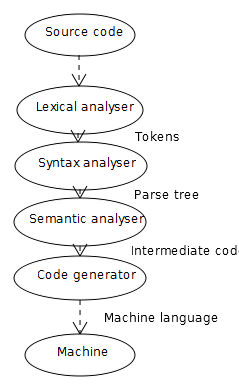
\includegraphics[scale=0.5]{pictures/compileroverview.png}
\capt{The different phases of a compiler. Based on Sebesta \textit{et al.}\cite{sebesta2013} p. 46, Figure 1.3}\label{fig:compileroverviewphases}
\end{figure}

\subsection{Lexical analysis}
The lowest level syntactic units of a language is called lexemes. A language's formal description does not often include these. They are instead described by a lexical specification, regular expressions i.e., separated from the syntactic specification\cite[p. 135]{sebesta2013}. Typical lexemes for a programming language includes integer literals, operators and special keywords like \textit{if} and \textit{while}. If both \textit{\$a} and \textit{\$b} are lexemes describing a variable and \textit{102} and \textit{42} are lexemes describing an integer, then \textit{\$a} and \textit{\$b} or \textit{102} and \textit{42} can typically be used interchangeably and still give a meaningful program. Therefore the lexemes are grouped into tokens. The name of a variable or the value of an integer is preserved when tokenising. The tokens are an abstraction that makes it easier to analyse if correct syntax of the language. An example of the grouping of lexemes into tokens can be seen by \tableref{table:lexandtokens}. After the lexical analysis an input stream of characters has been converted to an output stream of tokens.

\begin{figure}
\centering
\begin{table}
    \begin{tabular}{|l|l|l|l|l|l|l|l|}
        \hline
        Lexemes & \$a  & =      & 3   & \$b  & +    & 4   & \$a  \\ \hline
        Tokens & var & assign & int(3) & var(b) & plus & int(4) & var(a)  \\
        \hline
    \end{tabular}
\end{table}
\capt{Lexemes and their corresponding token group.\label{table:lexandtokens}
\end{figure}

\subsection{Syntax analysis}
All languages whether natural or artificial is a set of strings of characters over some alphabet. There are rules for how the strings can look that are in a language and how they can be combined. The lexemes described how the strings can look and now the tokens are useful when analysis how the lexemes can be combined. The rules can be specified formally to describe the syntax of a language\cite[p. 135]{sebesta2013}. A common way to describe a language's syntax is by a formal language-generation mechanism (also called grammars or context free grammars). By describing a grammar that can generate all possible strings in a language, the language has also been formally described. Backus-Naur Form is such a mechanism which in the 1950's became the most widely used method for describing programming language syntax\cite[p. 137]{sebesta2013}.
The BNF contains a set of terminals and a set of non-terminals. The terminals are the tokens from the lexical analysis. The non-terminals all have a set of productions, from which a mix of terminals and non-terminals can be derived from. A start production specifies a single non-terminal, from where all syntactically valid strings that are in the language can be derived from by using the production rules until only a sequence of terminals (the tokens) are left. The syntax analysis takes a sequence of tokens as input and tries to create a set of derivations from the start symbol that creates the given sequence of tokens. If success, the input has been parsed and the parse tree is kept for later analysis. The parse tree is the information concerning how the start symbol was derived into the sequence of tokens, which yields a tree structure. This tree is called an abstract syntax tree.

\begin{ebnf}
%Expressions
\grule{program}{\gter{print} expr}
\grule{expr}{\gter{(} \gcat term \gcat \gter{)} \gcat operator \gcat \gter{(} \gcat term \gcat \gter{)}}
\grule{operator}{\gter{=}}
\galt{\gter{>}}
\galt{\gter{<}}
\grule{term}{number}
\galt{expr}
\grule{number}{\textbf{any number}}
\end{ebnf}


\subsection{Semantic analysis}
Not all characteristics of programming languages are easy to describe with a BNF and some even cannot be described using a BNF. If a programming language allows a floating-point value to be assigned to an integer variable but not the opposite, this \textit{can} be expressed with a BNF but if all such rules should be specified in the BNF, it would increase the size of it remarkably. With increased size, the formal description gets more clumsy to look at and also increases the risk that an error is contained in the BNF.
The rule that all variables must be declared before being used is impossible to express in a BNF. That would require the BNF to remember things, particularly those variables it had seen before, which it cannot. The problem of remembering things also shows up when we start to concern about scope rules. Typically, a variable declared in one scope cannot be used outside that scope. The BNF cannot describe such problems that we describe as static semantics rules. It is named static because the analysis required to check the specifications can be done at compile-time rather than runtime\cite[p. 153]{sebesta2013}.
In this semantic analysis phase, the compiler can check for type rules by starting to decorate the parse tree from the syntactic analysis with types. If the non-terminal \textit{expr} derives into the terminals \textit{int} \textit{plus} \textit{int} \textit{semicolon}, it can be decorated with the \textit{int}-type, so the analysis can proceed further up the tree and check that the type of the \textit{expr} is legal. If the \textit{expr(int)} is derived from a \textit{expr} \rightarrow \textit{expr(int)} +  \textit{expr(bool)} production, the static semantic rules must determine if the programs semantic is wrong or it the boolean value can be converted to the integer values zero or one.

\subsection{Code generation}
Every compiler must focus the translation on the capability of a particular machine architecture. The targeted architecture can be virtual such as the Java Virtual Machine. Generally speaking, the code generation phase translates the program into instructions that are carried out by a physical processor. Whether the architecture is virtual or real the program code must be mapped into the processors memory. Typically, the overall translation is broken into smaller pieces, where smaller subtrees of the abstract syntax tree are translated into executable form one at a time. However, there many things that must be considered when translating, i.e. \textbf{instruction selection}, which concerns how an intermediate code representation from the abstract syntax tree is to be implemented. There are many different ways to implement the same functionality, but some might be carried out faster than other. The code generation phase must also deal with problems concerning \textbf{register allocation} and \textbf{code scheduling}. Register allocation is concerned with effectively using the registers so moving the same variables between registers and memory is minimised\cite[p. 521]{fischer2009}. The code scheduling is an important aspect with pipelined processors. The aim is to produce instructions that executes in a way such that the pipelined execution will not have to stall unnecessary\cite[p. 551]{fischer2009}. Some of the problems associated with the pipelined execution is solved by move apart instructions that will interlock\cite[p. 552]{fischer2009}.

\subsection{Interpretation}
A pure interpretation of a program lies at the opposite end (from compilation) regarding to methods of implementation. With this approach, which can be see, on \figref{fig:compileroverviewinterpretation}, no translation is performed at all. An interpreter is interpreting a program written in the targeted language. It acts like a virtual machine which instructions are statements of high level language. By purely using interpretation, a source code debugger can easily be implemented. Various errors that might occur can once they are detected easily refer to which place in the source code that caused the error. The debugging is eased because the interpreter works like a software implementation of a virtual machine, thus the state of the machine and the value of a specific variable can be outputted at any time when requested. This will of course lead to the disadvantage that an interpreter uses more space than a compiler. Further more, the execution speed of an interpreter is usually 10 to 100 times slower than that of a compiler \cite[p. 48]{sebesta2013}.

\begin{figure}
\centering
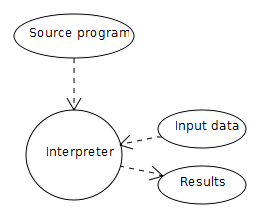
\includegraphics[scale=0.5]{pictures/compileroverviewinterpretation.png}
\capt{The different phases of an interpreter. Based on Sebesta \textit{et al.}\cite{sebesta2013} p. 48, Figure 1.4}\label{fig:compileroverviewinterpretation}
\end{figure}

The compiling or interpreting approach can be combined to form a hybrid implementation system. This method is illustrated in \figref{fig:compileroverviewhybrid}, where a program is compiled into an intermediate code which is then interpreted. By using this approach, errors in a program can be detected before interpretation which can save much time for a programmer. A great portability can also be achieved when using hybrid system. The initial implementation of Java was hybrid and allowed Java to be compiled to an intermediate code that could run on any platform which had an implementation of Java Virtual Machine\cite[p. 50]{sebesta2013}. 

\begin{figure}
\centering
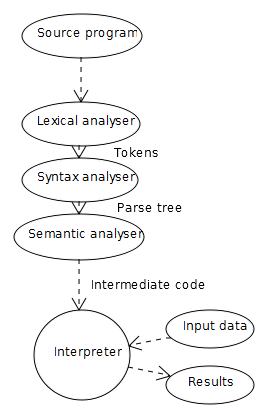
\includegraphics[scale=0.5]{pictures/compileroverviewhybrid.png}
\capt{The different phases of a hybrid implementation systems. Based on Sebesta \textit{et al.}\cite{sebesta2013} p. 49, Figure 1.5}\label{fig:compileroverviewhybrid}
\end{figure}